\subsection{Ozone mixing ratios as function of NOx and Temperature} \label{ss:r_contours}

\begin{figure}%
    \centering%
    \caption{Contours of maximum ozone mixing ratio as a function of the total \ce{NO_x} emissions on the first day and daily temperature for each chemical mechanism and using both a temperature-dependent and -independent source of isoprene emissions.}
    \label{f:ozone_contours}%
    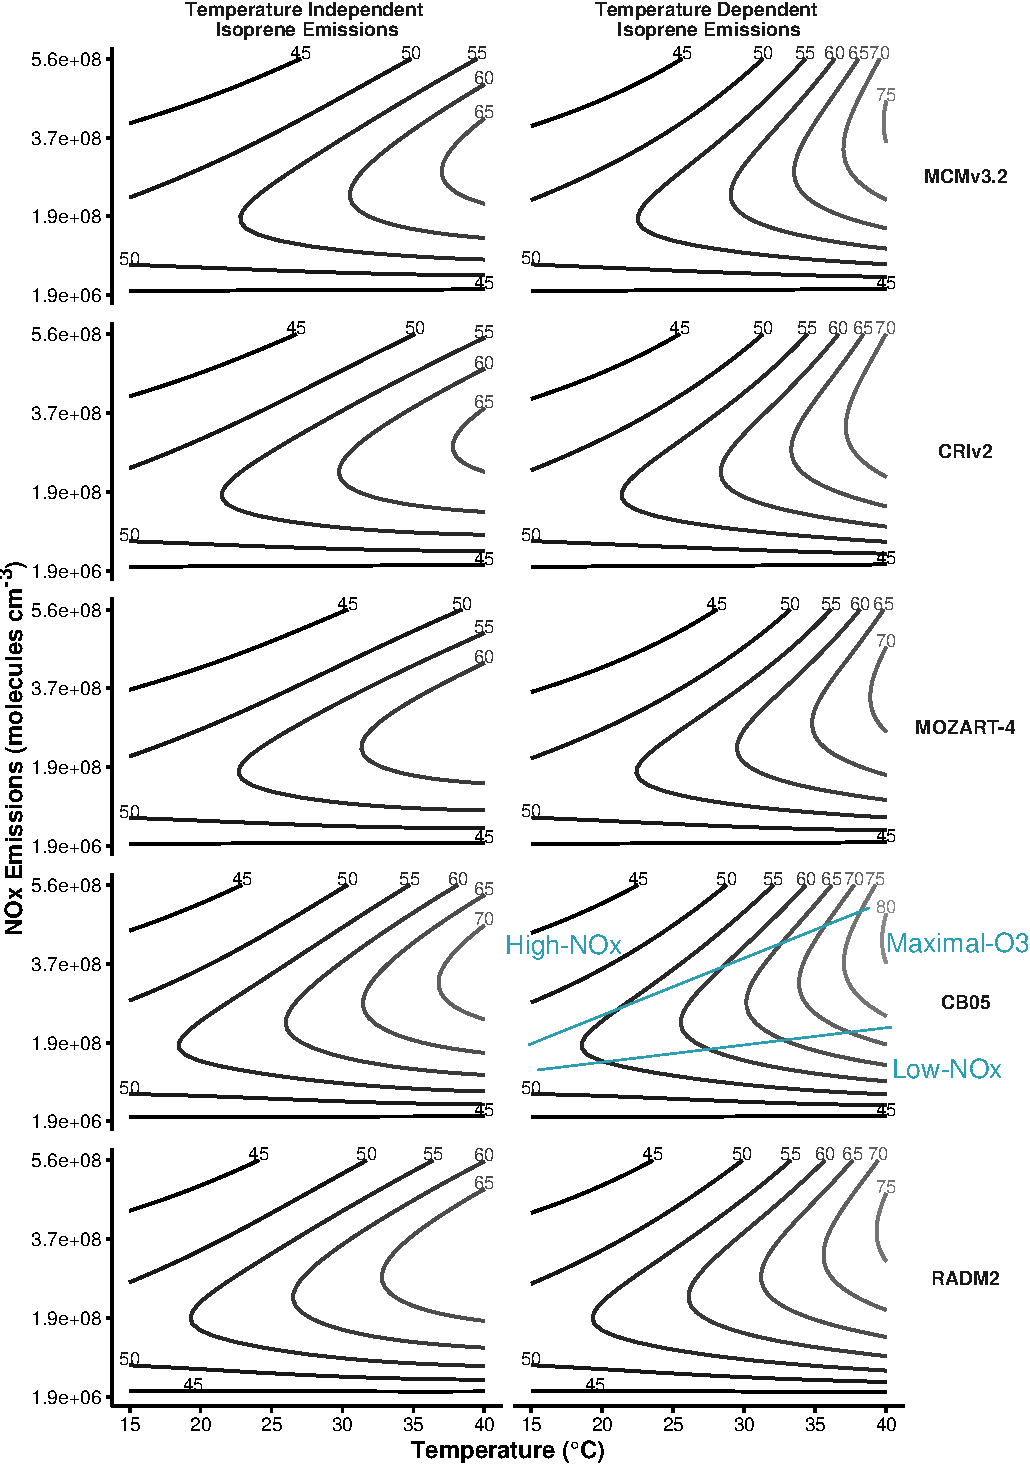
\includegraphics[width=\textwidth]{img/O3_comparison}
\end{figure}

\begin{figure}%
    \centering%
    \caption{Maximum 8-hr mean ozone mixing ratios at each temperature allocated to different \ce{NO_x} regimes. Slopes of linear correlation between ozone and temperature are also displayed for each chemical mechanism and source of isoprene emissions.}%
    \label{f:O3-T}%
    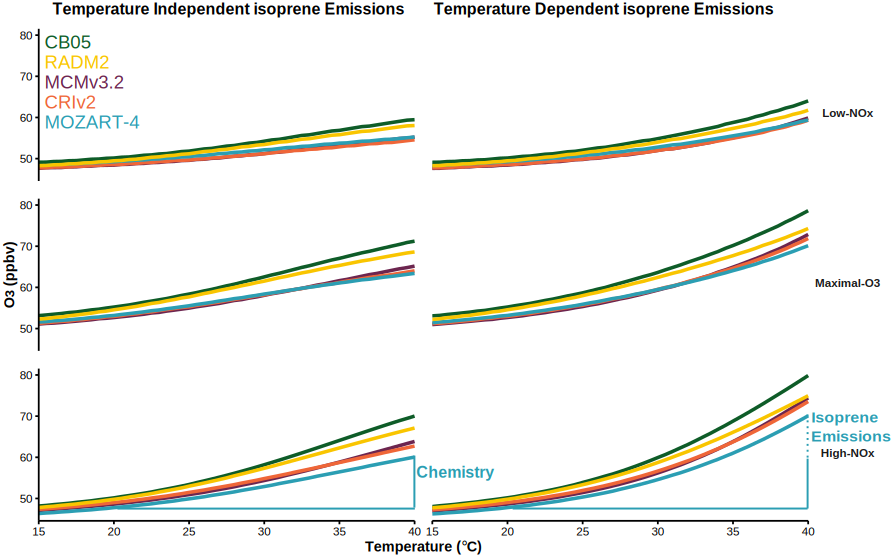
\includegraphics[width=\textwidth]{img/O3-T_correlation}%
\end{figure}

\begin{table}%
    \centering%
    \caption{Percentage increase in ozone mixing ratios at maximum temperature ($40$~$^{\circ}$C) from reference temperature ($20$~$^{\circ}$C) in Temperature Dependent and Independent Experiments.}%
    \label{t:difference_td_ti}%
    \begin{tabularx}{\textwidth}{c|c *{3}{|c}} 
    \hline \hline
    \textbf{Chemical} & \textbf{Source of} & \multicolumn{3}{c}{\textbf{Increase in Ozone from 20~$^{\circ}$C to 40~$^{\circ}$C (ppbv)}} \\ \cline{3-5}
    \textbf{Mechanism} & \textbf{Difference} & \textbf{Low-\chem{NO_x}} & \textbf{Maximal-\chem{O_3}} & \textbf{High-\chem{NO_x}} \\ 
    \hline \hline
    \multirow{2}{*}{MCMv3.2} & Isoprene Emissions & 4.6 & 7.7 & 10.6 \\ 
    & Chemistry & 6.8 & 12.5 & 15.2 \\ \hline
    \multirow{2}{*}{CRIv2} & Isoprene Emissions & 4.8 & 7.9 & 10.8 \\
    & Chemistry & 6.0 & 11.1 & 13.7 \\ \hline
    \multirow{2}{*}{MOZART-4} & Isoprene Emissions & 4.1 & 6.7 & 10.0 \\
    & Chemistry & 6.0 & 10.2 & 12.3 \\ \hline
    \multirow{2}{*}{CB05} & Isoprene Emissions & 4.6 & 7.4 & 9.8 \\
    & Chemistry & 9.3 & 16.0 & 19.9 \\ \hline
    \multirow{2}{*}{RADM2} & Isoprene Emissions & 3.8 & 5.7 & 7.8 \\ 
    & Chemistry & 8.6 & 14.1 & 17.3 \\
    \hline \hline
\end{tabularx}

\end{table}

Figure~\ref{f:ozone_contours} depicts the maximum mixing ratio of ozone obtained from each model run as a function of the total \ce{NO_x} emissions on the first day and temperature.
Using each mechanism, a similar non-linear relationship of ozone mixing ratios on \ce{NO_x} and temperature is found and increased ozone levels are found at higher temperatures when including a temperature-dependent source of isoprene emissions.
CB05 and RADM2 produce the largest amount of ozone at higher temperatures and higher \ce{NO_x} levels than the other chemical mechanisms.

The temperature-dependent source of isoprene leads to increased ozone mixing ratios at higher temperatures and higher \ce{NO_x} levels (top-right of each plot in Fig.~\ref{f:ozone_contours}).
The largest increase in ozone is found in the MCMv3.2 and CRIv2, where the ozone increased by 16~ppbv when using temperature-dependent isoprene emissions.
All other mechanisms, had similar increases in ozone with temperature-dependent isoprene emissions; RADM2 with an increase of 11~ppbv had the lowest increase in ozone.
At low temperatures, regardless of the \ce{NO_x} level, similar amounts of ozone are predicted from both the temperature-dependent and temperature-independent sources of isoprene emissions.

\subsection{Ozone budgets} \label{ss:r_budgets}

\begin{figure}%
    \centering%
    \caption{The contributions of the different reactions to total \ce{O_x} budget at each temperature at different \ce{NO_x} levels.}%
    \label{f:ozone_budgets}%
    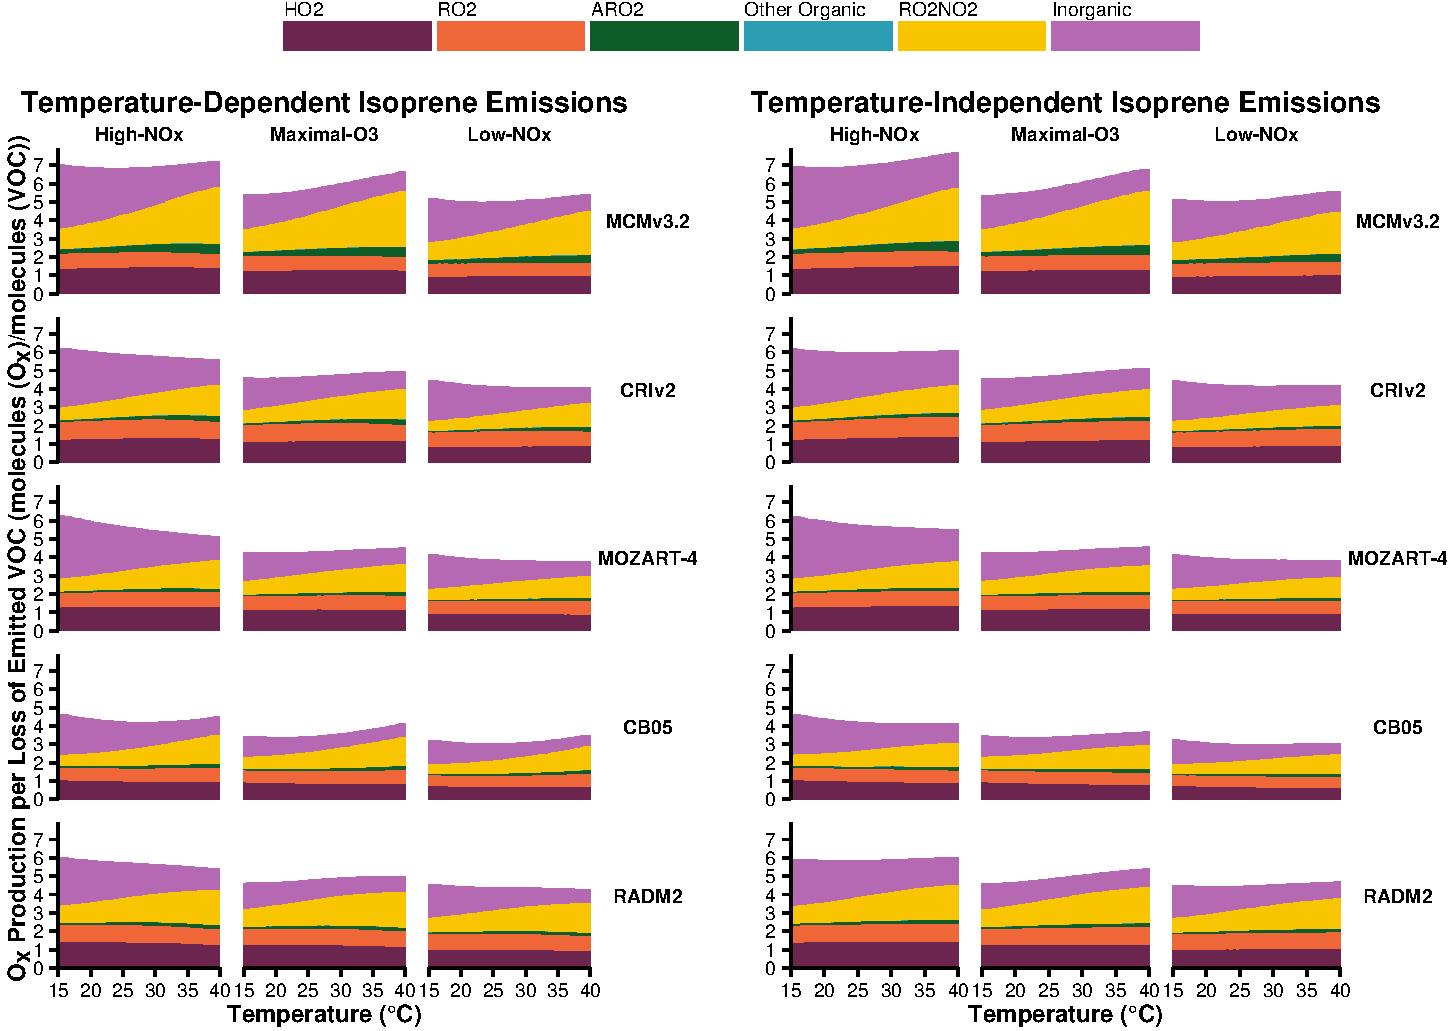
\includegraphics[width=\textwidth]{img/Ox_budgets}
\end{figure}

We defined the \ce{O_x} family to consist of \todo{complete this and reasons}

\citet{Sillman:1995} shows that the ratio of \ce{HNO3} to \ce{H2O2} can be used to determine whether an atmospheric system is in a \ce{NO_x}-sensitive, VOC-sensitive or in the ridge region of the \ce{NO_x}-VOC relationship with ozone, where maximum ozone is produced.
Based on this, we assigned each model run used to generate the ozone contours in Fig.~\ref{f:ozone_contours} to three \ce{NO_x} regimes--Low-NOx, High-NOx and Maximal-O3--corresponding to \ce{NO_x}-sensitive, VOC-sensitive and \ce{NO_x}-VOC-sensitive regions defined by \citet{Sillman:1995}.
Values of \ce{H2O2}/\ce{HNO3} less than $0.3$ correspond to the High-NOx regime, values larger than $0.5$ correspond to the Low-NOx regime and all values inbetween correspond to the ridge area in which maximal ozone is produced.

In Fig.~\ref{f:ozone_budgets}, the production rates on the first day of each reaction contributing to the \ce{O_x} production budget are determined and these reaction rates are then averaged over each \ce{NO_x}-condition (Low-\ce{NO_x}, High-\ce{NO_x} and Maximal-O3).
The fractional contribution of this reaction rate to the total \ce{O_x} budget was then calculated for each \ce{NO_x}-condition.

Figure~\ref{f:ozone_budgets} shows that the reaction of the hydroperoxyl radical (\ce{HO2}) with NO has the largest contribution at each \ce{NO_x}-condition, but this fractional contribution decreaes at higher temperatures due to the increased contributions of other reactions.
The increased contribution of the reaction of the acetyl peroxy radical (\ce{CH3CO3}) with NO with temperature has the most significant contribution to the total \ce{O_x} budget and this contribution is higher in CB05 and RADM2 compared to the other chemical mechanisms.

Add quantitative values of differences.

\subsection{Rate of Change of Ozone with Temperature} \label{ss:r_mO3-T}

\begin{figure}%
    \centering%
    \caption{Correlation of mean ozone mixing ratio with temperature in Low-NOx, maximal-O3 and High-NOx conditions for each chemical mechanism. A linear relationship between mean ozone mixing ratios and temperature is inferred, regression statistics are found in Table~\ref{t:O3_T_stats}.}%
    \label{f:rate_O3_T}%
    %\includegraphics[width=\textwidth]{img/Mean_O3_T_NOx_conditions}
\end{figure}

\begin{table}%
    \centering%
    \caption{Regression statistics for the linear relationship between ozone mixing ratios and temperature shown in Figure~\ref{f:rate_O3_T}.}%
    \label{t:O3_T_stats}%
    \scalebox{.78}[.78]{{\renewcommand{\arraystretch}{1.2}
\begin{tabular}{c|c|cc|cc|cc}
	\hline\hline
    \multirow{2}{*}{\textbf{Mechanism}} & \multirow{2}{*}{\textbf{Isoprene Emissions}} & \multicolumn{2}{c|}{\textbf{Low-\chem{NO_x}}} & \multicolumn{2}{c}{\textbf{Maximal-\chem{O_3}}} & \multicolumn{2}{|c}{\textbf{High-\chem{NO_x}}} \\
    & & \textbf{Mixing} & \textbf{No Mixing} & \textbf{Mixing} & \textbf{No Mixing} & \textbf{Mixing} & \textbf{No Mixing} \\
	\hline\hline
	\multirow{2}{*}{MCMv3.2} & Temperature Independent & 0.28 & 1.01 & 0.51 & 1.36 & 0.59 & 0.96 \\ 
    & Temperature Dependent & 0.42 & 1.48 & 0.74 & 2.16 & 0.93 & 2.63 \\ 
	\hline
	\multirow{2}{*}{CRIv2} & Temperature Independent & 0.25 & 0.93 & 0.47 & 1.27 & 0.55 & 0.88 \\ 
    & Temperature Dependent & 0.40 & 1.44 & 0.71 & 2.09 & 0.90 & 2.52 \\ 
	\hline
	\multirow{2}{*}{MOZART-4} & Temperature Independent & 0.25 & 0.97 & 0.44 & 1.21 & 0.49 & 0.59 \\ 
    & Temperature Dependent & 0.38 & 1.43 & 0.65 & 1.98 & 0.81 & 2.05 \\ 
	\hline
	\multirow{2}{*}{CB05} & Temperature Independent & 0.39 & 1.30 & 0.67 & 1.72 & 0.79 & 1.45 \\ 
    & Temperature Dependent & 0.52 & 1.72 & 0.89 & 2.44 & 1.12 & 2.94 \\ 
	\hline
	\multirow{2}{*}{RADM2} & Temperature Independent & 0.37 & 1.31 & 0.61 & 1.64 & 0.70 & 1.28 \\ 
    & Temperature Dependent & 0.48 & 1.68 & 0.79 & 2.22 & 0.97 & 2.49 \\ 
	\hline\hline
\end{tabular}}}

\end{table}

Each model run was allocated the three \ce{NO_x}-conditions as described in Sect.~\ref{ss:r_budgets} and then the mean ozone mixing ratio in these \ce{NO_x} regimes were then correlated with temperature as shown in Fig.~\ref{f:rate_O3_T}.
In literature, a linear relationship is typically reported between ozone and temperature and so the linear regression statistics are reported in Table~\ref{t:O3_T_stats}.

The linear increase of ozone with temperature, m$_{\text{O3-T}}$ in Table~\ref{t:O3_T_stats}, is highest at high-NOx conditions for each chemical mechanism and for each temperature case of isoprene emissions.
The high-NOx regime corresponds to the top regions of the contour plots in Fig.~\ref{f:ozone_contours} where increases in temperature would shift the ozone production towards the ridge of maximal ozone production, thus this increase in m$_{\text{O3-T}}$ is expected.
Similarly, the lowest m$_{\text{O3-T}}$ are achieved in the low-NOx regime, the bottom regions of the contours in Fig.~\ref{f:ozone_contours}, where increases in temperature do not neccisarily lead to increased ozone levels.
